%----------------------------------------------------------------------------------------
%	INTRODUCCIÓN (2,3 hojas)
%----------------------------------------------------------------------------------------

% Actualmente la realidad virtual tiene una variedad muy grande de dispositivos con diferentes características. Las principales especificaciones a tener en cuenta a la hora de decidir utilizar uno en concreto son la disponibilidad de accesorios como los mandos, la resolución de pantalla y los grados de libertad tanto de las gafas como de los periféricos, siendo típicos 3 y 6 grados.
% https://twitter.com/Diegobez/status/1038067397201207296
% https://twitter.com/Diegobez/status/925033415442919424








\pagestyle{empty}
\chapter{Introducción}
% tema de trabajo
La realidad virtual es una tecnología que desde hace unos años ha estado intentando hacerse un hueco en la industria del entretenimiento. Unity expuso estadísticas de consumo de realidad virtual durante el pasado año, proporcionando cifras como un 134\% de crecimiento en sobremesa y consola y un 295\% de crecimiento en las instalaciones de realidad virtual en móvil lo que hace casi un millón de usuarios a finales de 2017.

\begin{figure}[h]
\centering
\begin{subfigure}{.5\linewidth}
	\centering
	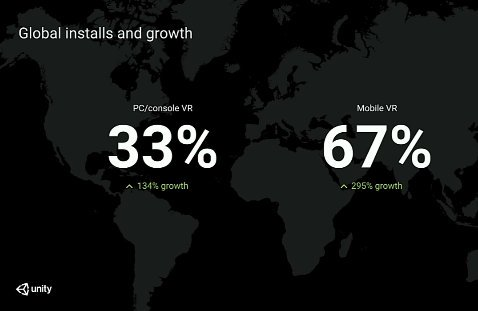
\includegraphics[width=0.90\linewidth]{Unite/global-installs.jpg}
\end{subfigure}%
\begin{subfigure}{.5\linewidth}
	\centering
	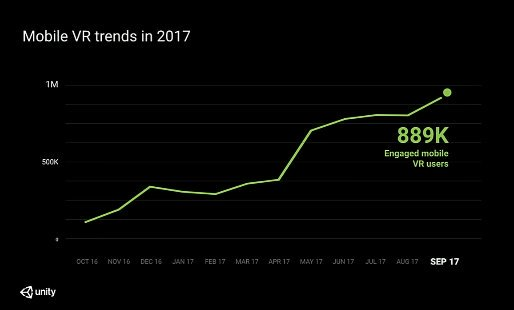
\includegraphics[width=0.97\linewidth]{Unite/mobile-trends.jpg}
\end{subfigure}
\end{figure}


\section{Grados de libertad}
Un factor clave a tener en cuenta cuando hablamos de realidad virtual son los grados de libertad, que definen la capacidad de movimiento a la hora de interactuar. Generalmente se habla de tres y seis grados de libertad. En el caso de tres grados de libertad, hace referencia a los giros sobre el eje principal (viraje o \textit{yaw}, inclinación o \textit{pitch} y cabeceo o \textit{roll}), mientras que cuando se amplia a seis grados de libertad hace referencia al desplazamiento en los tres ejes. Esto aplicado a las gafas de realidad virtual informa de la capacidad del dispositivo de captar los giros de la cabeza en todas las direcciones (tres grados de libertad) o si además capta el desplazamiento por la sala (seis grados de libertad).

El mercado de dispositivos de realidad virtual se está enfocando hacia seis grados de libertad. La alta gama ya dispone de ellos desde el principio mientras la gama media y baja ya está adaptándose como demuestra Oculus Santa Cruz o Vive Focus.

\section{Foto y vídeo en realidad virtual}
El contenido que se genera todavía esta basado en gran parte en técnicas ya conocidas como reproducción de vídeo y fotos cuya máxima adaptación consiste simplemente en poner una imagen ligeramente diferente en cada ojo.

La característica principal de este tipo de contenido es que cada imagen esta tomada desde un punto fijo en el espacio. Esto provoca una problemática que consiste en que el usuario únicamente tiene tres grados de libertad a la hora de visualizarlo en unas gafas de realidad virtual. Además de esta restricción debido a las técnicas de grabación que se usan, el cabeceo o \textit{roll} provoca ver imágenes duplicadas y puede provocar incomodidad o incluso mareo.

Debido a las estadísticas de consumo del contenido multimedia grandes empresas como Google, Facebook y Disney entre otras, están trabajando en mejorar los sistemas de visualización de vídeo y fotos mediante vídeo volumétrico, lightfields o fotogrametría.

La mayoría de proyectos que están disponibles actualmente utilizan técnicas que transforman cada frame en polígonos y desplazan los vértices en función de la profundidad que le indica un mapa de profundidad. Esto provoca en demasiadas ocasiones una deformación de elementos pequeños y en algunas ocasiones se ocultan elementos que deberían ser visibles de otro modo.

\section{Qué aporta este proyecto}
Este trabajo toma la demo ``Welcome to lightfields'' como referencia pero creando un proyecto de código libre. Trata de conseguir una sensación real de tres dimensiones habilitando seis grados de libertad en un espacio reducido de desplazamiento a partir de un vídeo estereoscópico plano en dos dimensiones y su mapa de profundidad. Para ello se hará un paralaje en tres dimensiones píxel a píxel en función del mapa de profundidad y la posición del usuario.

Durante el desarrollo del proyecto se llevan a cabo pruebas con diferentes técnicas y se evalúa la viabilidad en diferentes dispositivos (plataformas móviles y de sobremesa), el realismo del resultado así como la escalabilidad de los métodos.
















% interés
% Consumo de contenido
% Las gafas van a 6dof
% Hay gente que esta trabajando en ello (Facebook, Google)